\documentclass{article}
\usepackage[utf8]{inputenc}
\usepackage{amsmath}
\usepackage{minted}
\usepackage{tipa}
\usepackage{tikz}

\begin{document}
\def\sx{43} \def\sy{-55} \def\ex{55} \def\ey{-35}
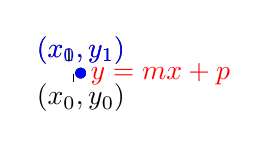
\begin{tikzpicture}[scale=0.125]
    \draw (\sx, \sy) node{$\bullet$} node[below]{$(x_0, y_0)$};
    \draw (\ex, \ey) node{$\bullet$} node[above]{$(x_1, y_1)$};
    \draw[blue] (\sx, \sy) -- (\sx, \ey) node{$\bullet$} node[above]{$(x_0, y_1)$};
    \draw[red] (\sx, \sy) -- (\ex, \ey) node[right,midway]{$y = mx+p$};
    \draw (\sx+0.25, \ey) -- (\sx+0.25, \ey+0.25);
    \draw (\sx+0.25, \ey+0.25) -- (\sx+0.25, \ey);
\end{tikzpicture}

\newpage
\begin{align*}
    \cos \theta &= \frac{\text{\color{blue}{adjacent}}}{\text{\color{red}{hypothénuse}}} \\
                &= \frac{| y_1-y_0|}{\sqrt{(x_1-x_0)^2 + (y_1-y_0)^2} } \\
    \text{ie}\quad \theta &= \arccos \left( \frac{| y_1-y_0|}{\sqrt{(x_1-x_0)^2 + (y_1-y_0)^2} } \right)   \\
    \text{ie}\quad \text{\texttheta } &= \text{\mint{python}|arccos(abs(y1 - y0) / sqrt((x1 - x0) ** 2 + (y1 - y0) ** 2)))|}
\end{align*}
\end{document}
